\documentclass{article}

\usepackage{url}
\usepackage{graphicx}
\graphicspath{{figs/}}
\usepackage{subfigure}

\usepackage[utf8]{inputenc}
\usepackage[ngerman]{babel}

\usepackage{booktabs}
\usepackage{multirow}
\usepackage{pifont}
\usepackage{color}
\newcommand{\cmark}{\ding{51}}%
\newcommand{\xmark}{\ding{56}}%

\begin{document}

%don't want date printed
\date{}

\title{Verteilte Systeme Aufgabe 1 Konzept}

\author{
  Marian Triebe, Moritz Heindorf\\
  %Dept. Informatik, HAW Hamburg, Germany\\
  \{marian.triebe, moritz.heindorf\}@haw-hamburg.de
}

\maketitle

\section{Analyse der Aufgabenstellung}
Mit Hilfe von CORBA sollen 2 verteilte Anwendungen implementiert werden. Diese sollen harmonisch mit den bereits vorhandenen Programmen, sowie den Programmen der Kommilitonen kommunizieren. Um die Programme möglichst unabhängig voneinander implementieren zu können steht ein IDL File bereit, welches die CORBA-Schnitstellen definiert. 

\section{Aufbau der Programme}
Die Programme bestehen aus den automatisch generierten Files (Servant, Skeleton) des IDL-Compilers, sowie der Implementierungen der Klassen `TruckCompanyImpl` und `CompanyImpl`. Beim Startup der Programme muss initial eine Referenz auf den Namensdienst sowie den RootPOA geholt werden. Dazu sind die entsprechenden CORBA-Calls auszuführen \textit{\tiny(ORB::resolve\_initial\_references(...)}, außerdem muss der ORB Dienst lokal initialisiert sein. Die Programme müssen danach eine Instanziierung ihrer Remote Objekte vornehmen, in unserem Fall enthält jede Programminstanz nur ein Remote Objekt. Die Remote Objekte müssen dann bei dem Namensdienst angemeldet werden, dazu Dient der beim Programmstart angegebene Company oder Truck Name. Es ist darauf zu achten, dass die Programme Ihre Remote Objekte korrekt beim Namensdienst abmelden, außerdem sind die korrekten Methoden aus der IDL aufzurufen, damit den anderen verteilten Anwendungen das beenden der Instanz signalisiert wird.

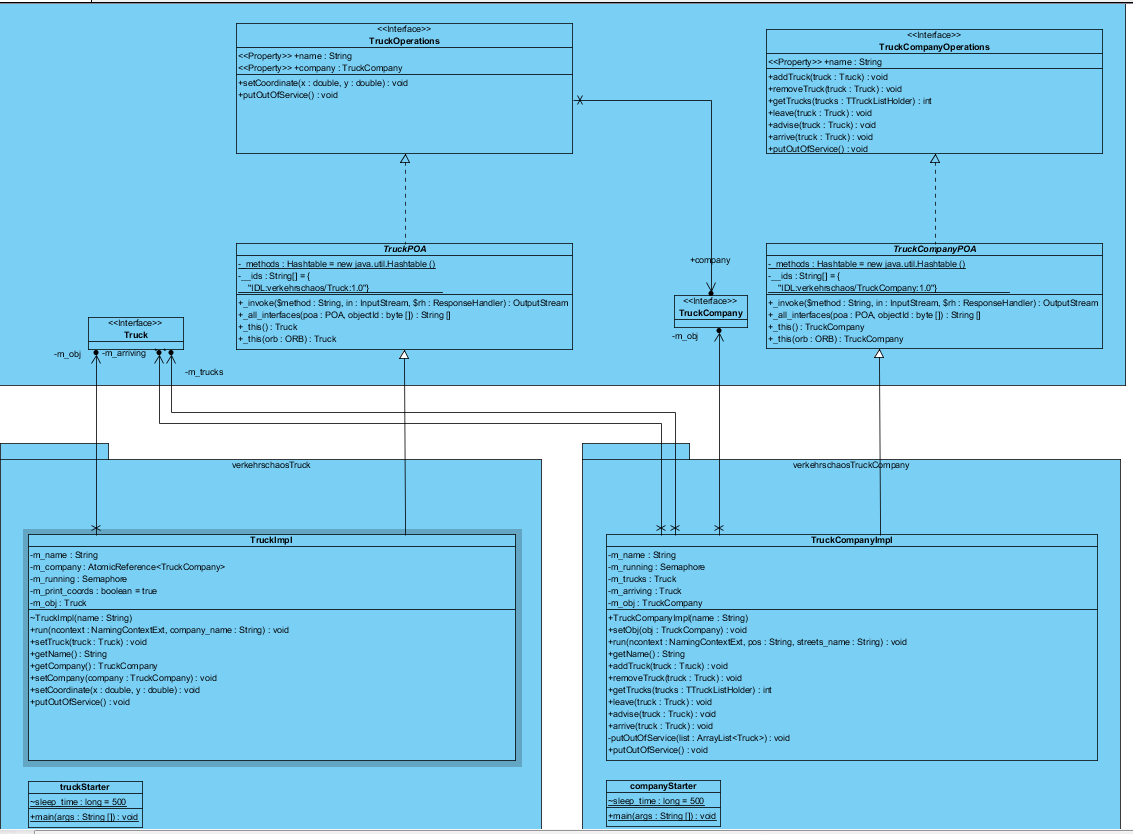
\includegraphics[scale=.4]{snapshot-2}
Das Klassendiagramm zeigt, wie im späteren Programm die jeweiligen `Impl` Klassen mit den automatisch generieten Interfaces/Klassen des IDL-Compilers arbeiten und/oder diese Implementieren. Außerdem gibt es eine Gesamtübersicht zur Kapselung der Datenstruktur der einzelnen Programme.

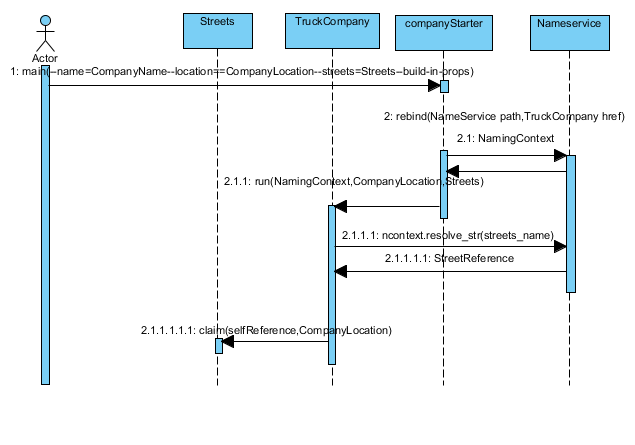
\includegraphics[scale=.7]{snapshot2}
Dieses Sequenzdiagramm verdeutlicht den späteren Ablauf des Company Programms. Es wird gezeigt, wie das CORBA-Objekt beim Namensdienst angemeldet wird. Rebind ist in diesem Kontext wichtig, falls sich ein Programm unter diesem Namen nicht korrekt vom Namensdienst abgemeldet hat. Jedoch könnte es unter umständen noch laufende Instanzen geben die diesen Namen beanspruchen. Außerdem wird gezeigt wie sich die Instanz des `Streets` Objekts geholt wird, dieses ist notwendig um die Company einem Platz zuzuordnen. Dazu wird auf dem Streets Objekt die Funktion \textit{\tiny claim(...)} aufgerufen.\\

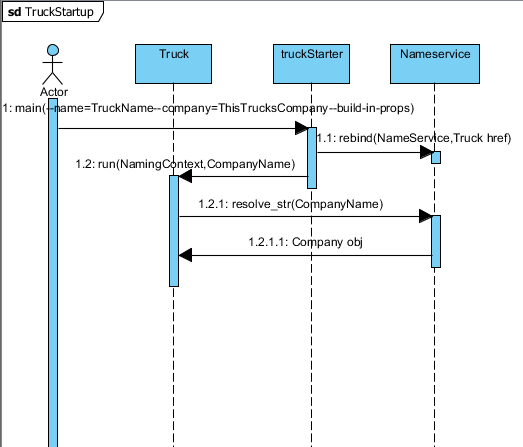
\includegraphics[scale=.75]{TruckStartup}

Dieses Sequenzdiagramm zeigt, wie im späteren Programm das Starten eines Trucks realisiert wird, der Ablauf ist ähnlich wie bei der Company Klasse, jedoch wird anstelle des `Streets` Objektes, ein Company Objekt vom Namensdienst abgerufen, welches beim Programmstart definiert wurde.

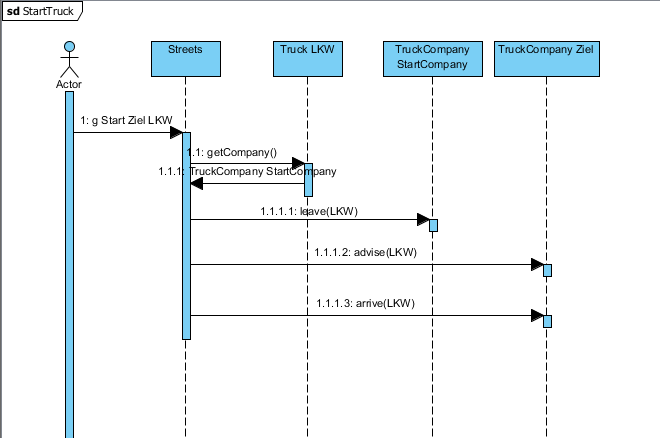
\includegraphics[scale=.7]{TruckMove}
In diesem Sequenzdiagramm ist zu sehen, wie von dem Konsolenprogramm aus ein Truck gestartet wird. Dazu wird `Streets` ruft dazu bei der Company die `leave` Funktion auf, diese ist ab dort nicht mehr für den Truck zuständig. Die Zielcompany bekommt den `advice` Aufruf von `Streets` und ist ab jetzt für den Truck zuständig.

\section{Mögliche Probleme}
\begin{itemize}
	\item Programme werden nicht richtig terminiert und melden sich nicht beim Namensdienst ab
	\item Nicht Thread sichere Programmierung, da die CORBA Calls in eigenen Threads auf den Remote-Hosts ausgeführt werden
	\item Löschen von Trucks die gerade auf dem Weg zu einer neuen Spedition sind
	\item Company Programme die beim terminieren Ihre Trucks nicht löschen, oder Ihre Position nicht freigeben
\end{itemize}

\end{document}
